%%%% CAPÍTULO 2 - REVISÃO DA LITERATURA (OU REVISÃO BIBLIOGRÁFICA, ESTADO DA ARTE, ESTADO DO CONHECIMENTO)
%%
%% O autor deve registrar seu conhecimento sobre a literatura básica do assunto, discutindo e comentando a informação já publicada.
%% A revisão deve ser apresentada, preferencialmente, em ordem cronológica e por blocos de assunto, procurando mostrar a evolução do tema.
%% Título e rótulo de capítulo (rótulos não devem conter caracteres especiais, acentuados ou cedilha)
\chapter{Referencial te\'orico}\label{cap:referencialTeorico}

Este capítulo apresenta os fundamentos teóricos que sustentam o desenvolvimento do agente proposto. 
São discutidos os conceitos de \gls{soc} e \gls{siem} na área de segurança da informação, as bases de conhecimento sobre vulnerabilidades e técnicas adversárias, o padrão \textit{Sigma} para regras de detecção, os modelos de linguagem de grande escala (\glspl{llm}), a geração aumentada por recuperação (\gls{rag}) e os agentes autônomos como paradigma de orquestração de \glspl{llm}.

\section{Segurança da Informação e SOC}

Em organizações de médio e grande porte a defesa cibernética não costuma ser tarefa de uma única ferramenta. 
O volume e a heterogeneidade dos eventos gerados por servidores, \textit{firewalls}, sistemas de detecção de intrusão (\gls{ids}), aplicações em nuvem e dispositivos de usuários tornam inviável a inspeção manual contínua, exigindo a composição de equipes e infraestruturas dedicadas ao monitoramento, à detecção e à resposta a incidentes \cite{vielberth2020soc, Shah2022}. É neste contexto que surgem os \gls{soc}, unidades especializadas que centralizam pessoas, processos e tecnologias para sustentar a postura defensiva de uma organização em tempo integral.

Segundo \citeonline{vielberth2020soc}, um \gls{soc} bem estruturado articula três pilares interdependentes: analistas humanos com diferentes níveis de experiência, procedimentos formalizados de triagem e resposta e uma camada tecnológica capaz de coletar, correlacionar e priorizar evidências de ameaças. 
A operação típica se organiza em níveis funcionais, em que no \textit{Tier} 1 os analistas iniciais executam a triagem dos alertas, no \textit{Tier} 2 os investigadores intermediários conduzem a análise de incidentes e no \textit{Tier} 3 os especialistas de nível mais alto realizam \textit{\gls{threat hunting}} e perícia forense \cite{tariq2025alert}. 
O componente tecnológico central que sustenta essa cadeia é o sistema \gls{siem}, descrito na próxima seção. 

\subsection{SIEM}

Um \gls{siem} atua como o núcleo de inteligência operacional em ambientes de cibersegurança, agregando e correlacionando \textit{logs} -- registros automáticos de eventos gerados por sistemas, aplicações, redes e dispositivos, provenientes de toda a infraestrutura de Tecnologia da Informação. 
Como já citado anteriormente, as fontes típicas incluem \textit{firewalls}, sistemas de detecção e prevenção de intrusão (\gls{ids}/\acrshort{ips}), servidores de aplicação e de banco de dados, controladores de domínio, \textit{endpoints} e serviços em nuvem \cite{gonzalez2021siem}. 
Seu propósito reside na capacidade de correlacionar eventos aparentemente desconexos e identificar padrões que ferramentas isoladas não o fazem.

Convém distinguir o \gls{siem} de outras soluções pontuais de defesa, como antivírus, \textit{firewalls} ou plataformas de proteção de \textit{endpoint} (\acrshort{epp}). 
Tais soluções operam de forma localizada -- protegendo um \textit{host}, um perímetro de rede ou um vetor específico, e geram alertas específicos de seu escopo. 
O \gls{siem}, por outro lado, é uma camada agregadora: ele consome os \textit{logs} produzidos por essas ferramentas, normaliza formatos heterogêneos para um esquema comum e aplica regras de correlação capazes de identificar, na conjunção de múltiplos eventos, padrões de ataque que permaneceriam imperceptíveis em uma análise isolada \cite{gonzalez2021siem, sheeraz2024siem}.
Conforme destacam \citeonline{PodzinsRomanovs}, essa contextualização é decisiva em ações automatizadas contra ameaças complexas, como ataques \textit{zero-day}, em que, por exemplo, a correlação entre uma tentativa de força bruta no \textit{Active Directory} (serviço de diretório da \textit{Microsoft} responsável pelo gerenciamento de identidades, recursos e permissões da rede interna) e um tráfego suspeito no \textit{firewall} pode disparar uma resposta imediata.

Nos \gls{soc}s, o \gls{siem} assume papel operacional indispensável: 
consolida alertas de diferentes fontes e formatos, prioriza incidentes com base na criticidade e orquestra fluxos de resposta (\textit{workflows}). 
Sem essa camada, os analistas perdem a capacidade de detectar fases avançadas de ataque, como movimento lateral e escalação de privilégios -- etapas em que o invasor se desloca pelos sistemas do alvo acumulando privilégios até atingir o nível administrativo \cite{PodzinsRomanovs}. 
A ausência desse tipo de visão integrada está associada a violações de longa duração, como foi o caso da rede mundial de hotéis \textit{Starwood}, em que a intrusão permaneceu não identificada por aproximadamente quatro anos e resultou no vazamento de dados de cerca de 383 milhões de hóspedes ao redor do mundo \cite{Marriot}. 
Essa visão unificada transforma o \gls{siem} no "sistema nervoso" do \gls{soc}, permitindo que analistas investiguem ameaças sistêmicas e não apenas alertas isolados.

A eficácia de um \gls{soc}, porém, está intrinsecamente ligada à robustez do \gls{siem} e à calibração das suas regras de detecção. 
Regras mal calibradas geram excesso de falsos positivos e instâncias não otimizadas podem produzir mais de mil alertas diários, sobrecarregando as equipes -- segundo \citeonline{PodzinsRomanovs}, um analista isolado consegue investigar com profundidade entre 5 e 15 alertas por dia, dependendo da criticidade. 
Esse desequilíbrio configura o fenômeno conhecido como \textit{alert fatigue}, ou fadiga de alertas: a exposição contínua a grandes volumes de notificações de baixo valor leva os analistas à dessensibilização, ao prolongamento do tempo de resposta e, em última instância, ao \textit{burnout} profissional, com impactos diretos na qualidade da defesa \cite{tariq2025alert}. 
A literatura recente identifica a fadiga de alertas como um dos principais desafios contemporâneos dos \gls{soc}s e, justamente por isso, motiva a busca por mecanismos automatizados de triagem, correlação e geração de regras mais precisas -- preocupação central do presente trabalho.

A importância estratégica do \gls{siem} também se ancora na sua capacidade de reduzir o tempo de detecção de ameaças. 
\citeonline{PodzinsRomanovs} citam o relatório de violações da \textit{Verizon} de 2018, que apontava cerca de 68\% das violações sendo descobertas meses ou mais após o ataque inicial \cite{verizon2018dbir}; 
já o relatório de 2025 informa que o tempo médio de remediação de vulnerabilidades em dispositivos de borda (especialmente falhas de \textit{zero-day}) é de 32 dias \cite{verizon2025dbir}. 
Essa lacuna pode ser substancialmente reduzida com um \gls{siem} bem implementado, em virtude da correlação de eventos em tempo real. 
Adicionalmente, a plataforma \gls{siem} serve de alicerce para a evolução tecnológica do \gls{soc}: é sobre ela que se integram componentes mais recentes, como módulos de inteligência artificial e aprendizado de máquina, que ampliam a detecção de ameaças sutis e habilitam a automação de respostas \cite{tendikov2024siem}.

Do ponto de vista econômico, embora o \gls{siem} envolva custos elevados -- com licenças baseadas em volume de \textit{logs}, infraestrutura dedicada e equipe especializada em regime ininterrupto, o investimento se justifica diante da magnitude das perdas associadas a incidentes cibernéticos. 
Em 2019, a \textit{Accenture} projetava perdas globais da ordem de US\$ 5,2 trilhões para os 5 anos seguintes \apud{accenture2019securing}{PodzinsRomanovs}, tendência que se confirmou nos anos posteriores: 
o relatório anual da IBM de 2024 (\cite{ibm2024costbreach}) registrou um custo médio global de US\$ 4,88 milhões por violação de dados, com aumento de 10\% em relação ao ano anterior. 
O último, de 2025, no entanto, trouxe uma pequena reviravolta: o custo médio global caiu 9\% em relação a 2024, motivado por melhorias na identificação e contenção de incidentes \cite{ibm2025costbreach}.
Para organizações com dados sensíveis ou sujeitas a regulações como o \gls{gdpr}, da União Europeia, ou o \acrshort{pci-dss} -- norma globalmente reconhecida para a segurança de dados de cartões de pagamento, o \gls{siem} deixa de ser uma opção e torna-se requisito operacional. 
Em síntese, o \gls{siem} mantém-se como pilar irrevogável da segurança corporativa, não apenas pela sua tecnologia isolada, mas por construir o ecossistema integrado de detecção e resposta sobre o qual se constroem as defesas modernas.

\subsection{SIEMs Inteligentes}

Apesar de sua centralidade operacional, o o sistema \gls{siem} tradicional opera majoritariamente sobre regras estáticas -- definições escritas por especialistas que descrevem condições de alertas a partir de padrões conhecidos. 
Essa abordagem apresenta duas limitações sistemáticas: a dificuldade em detectar ameaças cuja assinatura ainda não foi formalizada, como ataques \textit{\gls{zero-day}}, e a alta taxa de falsos positivos quando as regras não acompanham a dinâmica do ambiente protegido \cite{gonzalez2021siem, Nurusheva2024}.
\citeonline{gonzalez2021siem} observam, especificamente, que pouquíssimas soluções de \gls{siem} dispõem de mecanismos de correlação avançada capazes de realizar uma análise histórica e de desvios necessária, por exemplo, para a detecção posterior de ataques \gls{zero-day}. 
Portanto, é a partir da integração de técnicas de aprendizado de máquina \gls{ml} e \gls{ia}, buscando superar tais limitações, que se originam os chamados \gls{siem}s inteligentes.

De acordo com \citeonline{Saddi2024}, a \gls{ia} generativa é capaz de produzir dados sintéticos e simular cenários de ataque -- replicando, por exemplo, a atuação de um invasor ou a propagação de \textit{malware}, o que permite tanto treinar modelos de detecção quanto avaliar defesas antes de sua implantação, sustentando uma postura proativa de identificação de ameaças emergentes. 
Essa capacidade é amplificada por algoritmos de \gls{ml} que analisam padrões contextuais em grandes volumes de \textit{logs}, correlacionam eventos aparentemente desconexos -- por exemplo, tráfego anômalo combinado com tentativas de força bruta, e identificam comportamentos compatíveis com técnicas adversárias documentadas. 
\citeonline{tendikov2024siem} reforçam que a integração de \gls{ia} e \gls{ml} em \gls{siem}s aprimora a correlação de grandes volumes de eventos em tempo real e permite que esses sistemas aprendam a partir de dados históricos e se adaptem dinamicamente a ameaças emergentes. 
Esse aprimoramento incide diretamente sobre a fadiga dos analistas discutida na seção anterior: \citeonline{tariq2025alert} documentam que mecanismos de automação e triagem assistida por \gls{ml} reduzem a carga cognitiva associada ao alto volume de alertas e ao excesso de falsos positivos, principais causas do esgotamento nos \gls{soc}s.

\citeonline{Nurusheva2024} demonstram que algoritmos de detecção de anomalias, análise preditiva e limiares adaptativos permitem identificar atividades sutis que escapariam das regras estáticas ou à análise manual, e propõem um sistema autoadaptativo, capaz de identificar ameaças inéditas em tempo real sem depender de regras predefinidas. 
Um aspecto central desse paradigma é a possibilidade de reduzir a dependência de bases previamente rotuladas
\footnote{Uma base rotulada (do inglês \textit{labeled dataset}) condiz a uma coleção de pares entrada-saída, onde cada amostra de entrada (por exemplo, linha de \textit{log} ou fluxo de rede) recebeu uma anotação confiável sobre o que se é de fato}: 
como destacado por \citeonline{tariq2025alert}, algoritmos não supervisionados conseguem modelar o comportamento típico de uma rede e detectar anomalias sem a necessidade de conjuntos de dados rotulados, o que os torna particularmente eficazes na identificação de ameaças novas -- embora ao custo de uma taxa de falsos positivos superior à dos métodos supervisionados. 
Do ponto de vista conceitual, esse comportamento decorre das próprias características do aprendizado de máquina, cuja capacidade de aprender padrões a partir de dados, sem programação explícita, fundamenta tanto as abordagens supervisionadas quanto as não-supervisionadas \cite{jordan2015machine}. 
Ao combinar esses dois tipos de modelo, o \gls{siem} com \gls{ml} ajusta-se continuamente às mudanças no ambiente e antecipa novos vetores de ataque \cite{sheeraz2024siem}.

%Uma materialização particularmente difundida dessa abordagem é o conjunto de técnicas designadas como \gls{ueba}, em que perfis de usuários e entidades são construídos automaticamente a partir do histórico de eventos e usados para sinalizar desvios estatisticamente significativos em relação a uma linha de base de comportamento normal (HASSAN et al., 2025). 
%No arcabouço descrito por Hassan et al. (2025), por exemplo, o módulo UEBA emprega exclusivamente algoritmos não supervisionados — especificamente o Isolation Forest —, opção justificada precisamente pela escassez de sessões maliciosas rotuladas em operações reais. O UEBA costuma compor, junto ao SIEM, plataformas integradas que incluem ainda módulos de orquestração e resposta automatizada (Security Orchestration, Automation, and Response, SOAR), capazes de executar ações de contenção — como reforço de autenticação, isolamento de endpoints e bloqueio de endereços IP — com mínima intervenção humana (HASSAN et al., 2025).

Por fim, compreende-se que depender exclusivamente de analistas humanos é inviável diante do crescimento exponencial dos dados e da sofisticação das ameaças. 
A incorporação de \gls{ia} e \gls{ml} em \gls{siem}s representa, portanto, um avanço significativo da cibersegurança, conferindo precisão, adaptabilidade e automação a um cenário cada vez mais dinâmico e hostil. 
Esse movimento, no entanto, ainda enfrenta desafios relevantes, sobretudo no que tange à interpretabilidade dos modelos, à dependência de dados de qualidade para o treinamento e à necessidade de regras formais que estabeleçam o vocabulário comum entre as diferentes ferramentas. 
Seguindo este último ponto, nas próximas seções se discutirá sobre a efetividade de qualquer \gls{siem}; sendo inteligente ou não, depende de regras de detecção formalizadas em padrões abertos e interoperáveis, ancoradas em bases consolidadas de conhecimento sobre vulnerabilidades e técnicas adversárias.


\section{Bases de Padrões de Ataques}

Para a criação de regras em SIEMs, assim como para qualquer tipo de regra, há de se adotar algum padrão.
No mundo da cibersegurança existem padrões que catalogam e identificam vulnerabilidades, eventos e outras categorias do gênero. 
Duas categorizações são o CVE e o CWE.
O CVE --- \textit{Common Vulnerabilities and Exposures} (Vulnerabilidades e Exposições Comuns), é um programa mantido pelo MITRE desde 1999, que define e cataloga vulnerabilidades e exposições de segurança publicamente conhecidas, no qual se atribui um identificador único (CVE-ID) e padrão para cada uma.
Atualmente possuindo quase 300 mil registros, o CVE é uma referência confiável para integrar bancos de dados de segurança, alertas, produtos comerciais e soluções automatizadas \cite{NIST_CVE_Process, CVE_History}.

Já o CWE --- \textit{Common Weakness Enumeration} (Enumeração de Fraquezas Comuns), também mantido pelo MITRE, é um catálogo comunitário de tipos de fraquezas (como falhas de validação, \textit{buffer overflow}, injeção), usadas para identificar a causa raiz subjacente às vulnerabilidades. 
Quando um CVE descreve um ``\textit{buffer overflow}'', ele pode ser correlacionado a um CWE específico, permitindo que os analistas entendam quando se trata de um erro de lógica, design ou implementação \cite{CWE_About, CWE_Usage_Guidance}.

O MITRE, que mantém as duas listagens citadas acima, é uma organização sem fins lucrativos, mantida por agências como o NIST (Instituto Nacional de Padrões e Tecnologia, do inglês \textit{National Institute of Standards and Technology}) 
e CISA (Agência de Segurança Cibernética e Infraestrutura, do inglês \textit{Cybersecurity and Infrastructure Security Agency}). 
Além da contribuição citada acima, o MITRE criou uma solução alternativa chamada MITRE ATT\&CK --- 
uma base de dados sobre táticas e técnicas adversárias, acessível globalmente, baseada em observações do mundo real. 
É usada como base para o desenvolvimento de modelos e metodologias de ameaças no setor privado, governo e na comunidade de produtos e serviços de cibersegurança \cite{MITRE_ATTACK}.
A base é aberta e está disponível gratuitamente para uso de qualquer indivíduo ou organização, assim como o CVE e CWE. 

Não menos importante é o NVD --- \textit{National Vulnerability Database} ou Base Nacional de Dados de Vulnerabilidades, repositório do governo dos EUA e mantido pelo NIST.
É responsável por armazenar dados padronizados sobre vulnerabilidades de segurança seguindo o protocolo SCAP (\textit{Security Content Automation Protocol}. 
O repositório inclui listas de falhas em \textit{softwares}, métricas de impacto, nomes de produtos, configurações vulneráveis e \textit{checklists}, permitindo automação da gestão de vulnerabilidades, avaliação de segurança e conformidade \cite{NIST_NVD_General}. 

Esses elementos são pilares para as regras de SIEMs/\textit{Sigma}, pois fornecem contexto de acionamento e padronização. 
O NVD enriquece CVEs com dados de severidades (como o CVSS (\textit{Common Vulnerability Scoring System}), método usado para fornecer uma medida qualitativa de gravidade \cite{NIST_NVD_Metrics})
e produtos afetados, permitindo que SIEMs priorizem alertas com base no risco real. 
As classificações CWE ajudam a desenvolver regras \textit{Sigma} para fraquezas comuns, detectando ataques mesmo quando variantes novas surgem.
Já o mapeamento MITRE entre CWE e CVE vincula falhas de código a vulnerabilidades exploradas, refinando a correlação de ameaças em SIEMs. 
Por exemplo, uma regra \textit{Sigma} pode usar o CWE-352\footnote{Falsificação de solicitação entre sites, do inglês \textit{Cross-Site Request Forgery} (CSRF) \cite{CWE_352}.} 
para monitorar solicitações não autorizadas, enquanto o CVE associado direciona \textit{patches} críticos \cite{nist_cwe_slice}.

\section{Regras \textit{Sigma}}

Sigma (\textit{Generic Signature Format for SIEM Systems}, ``Assinatura em formato genérico para sistemas SIEM'' em tradução livre \cite{SigmaReadMe}) 
é o projeto de código aberto de um padrão genérico de descrição de \textit{logs} de eventos, aplicável a qualquer tipo de \textit{log},
com o intuito de compartilhar a lógica de detecção de ameaças ou anomalias entre diferentes SIEMs. 
Ao operar com dados de ameaças de múltiplas fontes, o \textit{Sigma} capacita os caçadores de ameaças a correlacionar eventos que passariam despercebidos por abordagens convencionais. 
Dessa forma, se obtém conhecimentos estratégicos sobre dados confiáveis e antecipa-se tentativas de ataque em estágios iniciais desta cadeia de eventos \cite{Splunk1}.

Os mantenedores da iniciativa consideram que excelentes análises podem ser encontradas na \textit{internet}, incluindo IOCs e regras YARA\footnote{Uma regra YARA é um arquivo de extensão ``.yar'' contido de expressões lógicas usadas para classificar e identificar amostras de \textit{malware} \cite{PicusSecurity}.} para detectar arquivos ou ferramentas maliciosos, por exemplo, mas que muitas vezes limitam-se a descrições específicas, funcionais para poucos \textit{softwares}.
Portanto, da necessidade de haver um método de descrição específico ou genérico de eventos de \textit{logs}, com portabilidade para vários SIEMs, a fim de aprimorar os recursos de detecção para todos, surgiu o Sigma \cite{SigmaReadMe}.

O projeto de código aberto foi criado em 2017 por Florian Roth e Thomas Patzke \cite{AboutSigma}, inspirados em padrões já existentes nas áreas de análise de \textit{malware} e monitoramento de rede. Como já dito, o padrão \textit{Sigma} se diferencia por lidar com vários tipos de esquemas de \textit{logs}, unindo padrões que já existem e se diferenciam entre si \cite{Splunk1}. 

O projeto carrega essa denominação pois se considera um ecossistema --- envolve três componentes: o formato \textit{Sigma}, a ferramenta \textit{Sigma} e a coleção de regras \textit{Sigma}. 
Este último diz respeito ao repositório no \textit{Github}, que possui mais de 3 mil regras de detecção de diferentes tipos; 
por ser de código aberto, pode receber sugestões de qualquer pessoa disposta a contribuir \cite{SigmaReadMe}. 
Já a ferramenta \textit{Sigma}, refere-se a um conversor de regras disponível para \textit{download} --- o \textit{Sigma Command Line Interface} (CLI). 
Com ele é possível converter as regras \textit{Sigma} para as regras usadas no SIEM de interesse do usuário; 
\textit{Elasticsearch}, \textit{CrowdStrike}, \textit{IBM QRadar AQL} e \textit{Splunk} são algumas marcas registradas para as quais essa integração está disponível.

\subsection{Sigma e a mitigação de ameaças}

As regras \textit{Sigma} formam um conjunto estruturado de princípios e métodos essenciais para o sucesso da investigação focada em determinar as ameaças que podem prejudicar um ou mais sistemas (\textit{Threat Hunting}), 
oferecendo um padrão uniforme que orienta os profissionais de segurança na elaboração de regras criteriosas para detecção de ameaças ou anomalias. 
Segundo \citeonline{Dimitrov2025YARA}, essas regras otimizam a identificação, avaliação e a resposta a incidentes,
proporcionando decisões mais precisas e oportunas, além de uma base sólida para controlar vetores de ameaças, minimizar riscos e prevenir violações de dados.
Dessa forma, as regras \textit{Sigma} constituem o alicerce de uma estratégia de segurança proativa e resiliente, capaz de antecipar e mitigar possíveis ataques de forma sustentável.

A caça a ameaças é um processo defensivo proativo que visa descobrir e neutralizar invasores, mapeando vulnerabilidades e antecipando movimentos adversos por meio da análise contínua de comportamentos anômalos e incidentes em curso.
Nesse cenário, as regras \textit{Sigma}, desde sua padronização, em 2017, desempenham um papel fundamental ao oferecer uma linguagem comum para correlação de eventos em múltiplas plataformas SIEM,
unificando dados de sistemas heterogêneos e acelerando a detecção de padrões suspeitos.
Conforme demonstrado por \citeonline{Dimitrov2025YARA}, essa unificação reduz significativamente a carga de trabalho manual dos analistas, 
permitindo identificar ameaças ainda na fase inicial de comprometimento, elevando a eficácia das operações de \textit{Threat Hunting}, ou ``caça a ameaças''.

No entanto, ainda que a aplicação das regras \textit{Sigma} viabilize inúmeros cenários benquistos, vale ressaltar que, ainda assim, os SIEMs continuarão sendo heterogêneos, pois utilizam formatos e padrões de dados diferentes --- situação inclusive de eventos de diferentes dispositivos. 
As regras \textit{Sigma} surgem como uma forma de expressar a regra ou a ameaça e o que deve ser buscado, mas ainda precisa ser convertida para o SIEM de destino (através do CLI), que já possui suas próprias regras.

\subsection{Estrutura}

As regras \textit{Sigma} são arquivos YAML contidos de informações que viabilizam a detecção de comportamento estranho ou malicioso quando da inspeção de arquivos de \textit{logs} dentro do contexto de um SIEM \cite{SigmaRules}. 

A compreensão da estrutura de uma regra \textit{Sigma} e como é usada para detecção faz-se importante em razão de que parte da metodologia envolverá selecionar as informações mais críticas das regras e avaliá-las.

As regras são divididas em três grupos principais de instruções \cite{SigmaRules}: 
\begin{itemize}
    \item Detecção (\textit{detection}): qual comportamento malicioso a regra está procurando;
	\item Fonte do log (\textit{logsource}): quais tipos de logs a detecção deve procurar; e
    \item Metadados (\textit{title}, \textit{id}, \textit{status}, etc.): detalhes da regra. 
\end{itemize}

A Figura \ref{fig:figura1} é um exemplo de regra \textit{Sigma} que está disponível na página oficial do projeto.  

\begin{figure}[htb]
    \caption{Exemplo de regra \textit{Sigma} \cite{SigmaRules}} 
	\label{fig:figura1}
    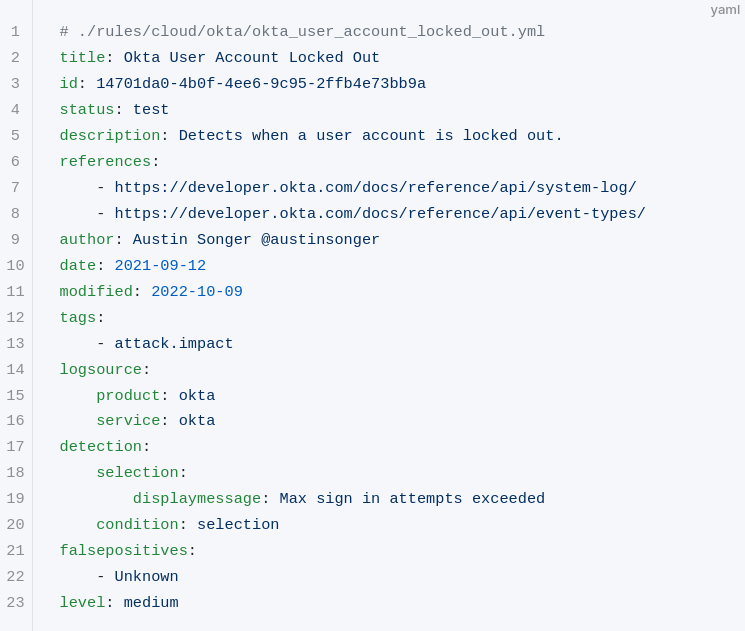
\includegraphics[scale=0.45]{figuras/figura 1.png}
	\fonte{Captura de tela da página \textit{Sigma Rules} em \citeonline{SigmaRules}}%% Fonte
\end{figure}

A seção de detecção é o coração da regra \textit{Sigma}, pois especifica o alvo da regra no vasto volume de \textit{logs}. 
Adiante neste trabalho este componente será mencionado como um dos principais para a análise da qualidade das regras geradas pelas IAs. 
Vale mencionar que, dentro da seção de detecção, existem instruções para a escrita, assim como qualquer linguagem de programação; 
no entanto, num primeiro momento, basta compreender o esqueleto principal. 
Sendo assim, a segunda peça mais importante da regra é a fonte dos \textit{logs}, o campo \textit{logsource}; 
nele se especifica qual o tipo de \textit{log} deve ser canalizado pela regra --- ao invés de varrer todos os \textit{logs} do SIEM. 
Por fim, as demais informações, os metadados, servem para guiar o usuário sobre o assunto da regra \cite{SigmaRules}. 

Para fins de orientação quando da criação de uma nova regra, é disponibilizado um esqueleto da regra com instruções (Figura \ref{fig:figura2}) no repositório \textit{Sigma} \cite{RuleCreationGuide}. 

\begin{figure}[htb]
    \caption{Exemplo de regra \textit{Sigma} \cite{RuleCreationGuide}} 
	\label{fig:figura2}
    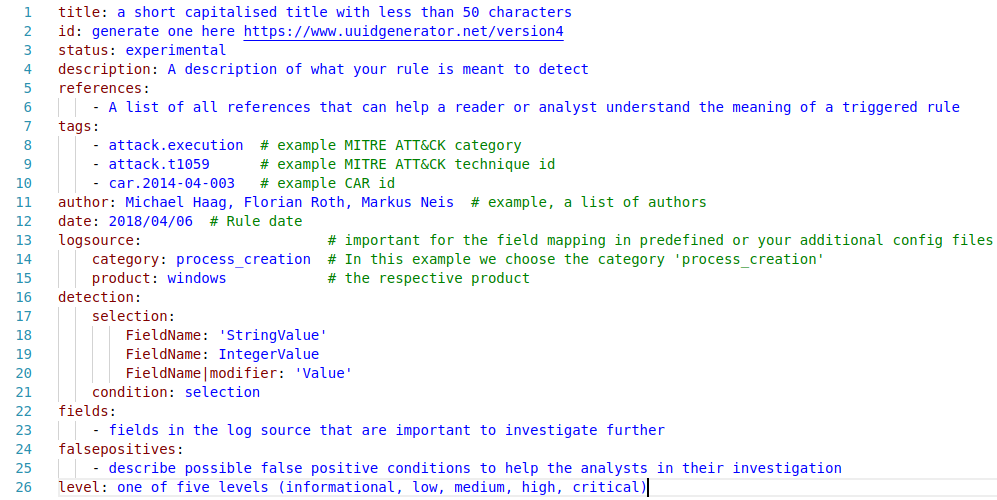
\includegraphics[scale=0.45]{figuras/figura 2.png}
	\fonte{Captura de tela do código genérico na página \textit{Rule Creation Guide} no repositório Sigma\cite{RuleCreationGuide}}%% Fonte
\end{figure}
    

\section{Processamento de Linguagem Natural}

Segundo \citeonline{liddy2001natural}, o Processamento de Linguagem Natural (PLN) é definido como uma abordagem computacional teórica e tecnológica fundamentada para analisar textos em linguagem humana. 
Seu objetivo central é alcançar um processamento linguístico semelhante ao humano, através da representação de textos aos níveis linguísticos:  
fonológico (padrões de entonação e fonemas), morfológico (estrutura das palavras), léxico (significado individual das palavras), sintático (estrutura gramatical das frases), semântico (significado literal das frases), discursivo (coesão e estrutura dos textos) e pragmático (contexto);
ou seja, o PLN fragmenta o texto e analisa sistematicamente as sete camadas citadas \cite{liddy2001natural, Chowdhary2020}.

As técnicas de PLN evoluíram de métodos simbólicos, baseados em regras e lógica formal, para abordagens estatísticas e conexionistas (ou seja,  inspirada no funcionamento do cérebro humano),
impulsionadas pelos avanços computacionais e a disponibilidade de coleções extensas e estruturadas de textos \cite{liddy2001natural}.

O PLN suporta aplicações críticas como a Recuperação de Informação (RI), Extração de Informação (EI), Tradução Automática (TA) e Sistemas de Pergunta-Resposta. 
\citeonline{liddy2001natural} cita um exemplo de RI em que sistemas PLN melhoraram a precisão em representar consultas e documentos em diversos níveis semânticos.
A EI utiliza reconhecimento de entidades e análise parcial para estruturar dados de textos não estruturados, como em anúncio de emprego.
Já os sistemas de diálogo, embora ainda dependentes de dimensões fonético-léxicas, buscam incorporar todas as camadas linguísticas para resultados mais naturais.
A sumarização automatizada --- geração de resumos concisos e coerentes a partir de textos extensos, aplica análise discursiva para condensar os textos enquanto mantém coerência \cite{Chowdhary2020, liddy2001natural}.

Alguns dos obstáculos do PLN envolvem a integração de conhecimento de mundo e raciocínio de senso comum, essenciais para resolver ambiguidades contextuais complexas.
Avanços nos modelos híbridos e ferramentas aceleram os experimentos, mas a compreensão profunda permanece distante, pois exige bases de conhecimento amplas e técnicas como inferência abdutiva para superar lacunas de interpretação \cite{Chowdhary2020}. 


\subsection{Modelos de Linguagem de Grande Escala (LLMs)}

Os Grandes Modelos de Lingugagem, do inglês \textit{Large Language Models} (LLMs),
são sistemas de inteligência artificial treinados com bilhões ou trilhões de parâmetros,
capazes de compreender e gerar textos em linguagem natural, ou seja, no formato de comunicação humano.
A arquitetura desses modelos é baseada em ``\textit{Transformers}'' --- redes neurais baseadas em mecanismos de \textit{self-attention} 
que permitem que o modelo foque em diferentes partes do texto simultaneamente, adquirindo relações contextuais de longo alcance entre as palavras \cite{weber2024redpajamaopendatasettraining};  
estes aprendem em grande escala através do aprendizado auto supervisionado (\textit{self-supervised learning}), extraindo padrões de grandes corpos de textos sem rótulos explícitos \cite{hasanov2024application}.
A evolução dessas redes marca um avanço na capacidade das máquinas ``entenderem'' contexto e intenção.

>>>>>>>>>>>>>>>>>>>>\citeonline{motlagh2024llmcyber} explica que o mecanismo central de um LLM se baseia na predição de \textit{tokens} (menores unidades de texto que um modelo de linguagem divide para processar) sequenciais: 
dada uma sequência de entrada, o modelo estima a probabilidade do próximo elemento textual, refinando essa habilidade ao longo do pré-treino.
Além disso, explica que técnicas como a ``\textit{in-context learning}'' permitem que o mesmo modelo execute tarefas específicas apenas com os exemplos fornecidos pelo \textit{prompt}, sem haver necessidade de ajuste fino. 
Esse paradigma torna possível a aplicação do mesmo modelo de LLM em diferentes tarefas sem precisar retreiná-lo \cite{motlagh2024llmcyber}.

>>>>>>>>>>>>>>>>>>>>>A aplicabilidade dos LLMs é vasta: auxiliam na geração de código, criação de conteúdos, atendimento ao cliente, análise de sentimentos e suporte à decisão clínica, entre outras funções \cite{motlagh2024llmcyber}. 
Contudo, desafios sempre existirão, e o alto custo computacional é um deles, além da tendência de reprodução de vieses presentes nos dados originais e vulnerabilidade a ataques de \textit{jailbreak}\footnote{Processo de exploração de falhas de um dispositivo eletrônico bloqueado para instalar outro \textit{software} que não o disponibilizado pelo fabricante para uso no dispositivo \cite{kaspersky2024jailbreaking}.}
e injeção de \textit{prompt}\footnote{Ocorre quando \textit{prompts} do usuário alteram o comportamento ou a saída do LLM de maneiras não intencionais. 
Essas entradas podem afetar o modelo mesmo que sejam imperceptíveis para humanos. Portanto, as injeções de \textit{prompt} não precisam ser visíveis/legíveis para humanos, desde que o conteúdo seja analisado pelo modelo. \cite{owasp2024promptinjection}}.
Superar qualquer entrave exigirá trabalho contínuo, transparência dos dados e aperfeiçoamento incessante das técnicas de mitigação de riscos. 


\subsection{Arquitetura \textit{Transformer}}



\subsection{Engenharia de \textit{Prompt}}



\section{Geração Aumentada por Recuperação (RAG)}



\subsection{\textit{Embeddings} e Bancos de Dados Vetoriais}



\subsection{RAG aplicado à Cibersegurança}



\section{Agentes Autônomos}



\subsection{Padrão \textit{ReAct}}



\subsection{\textit{LangGraph} como \textit{Orquestrador}}